\newpage
\section{Revisão da Teoria}

\subsection{Modulação PAM}

Modulação por amplitude de pulso (\textit{Pulse Amplitude Modulation} - PAM) é a maneira mais simples de modulação digital. Essa técnica consiste em transmitir dados através da variação da amplitude da tensão (ou potência) de um sinal pulsado, ou seja, a informação a ser transmitida é inserida na amplitude de uma sequência de pulsos elétricos, como mostra a figura \ref{fig:pam}. 

\begin{figure}[H]
    \centering
    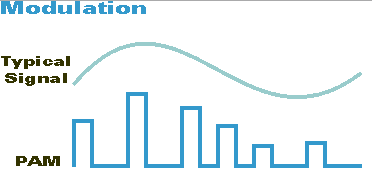
\includegraphics[scale=0.7]{pam}
    \caption{Modulação PAM de um sinal senoidal.}
    \label{fig:pam}
\end{figure}

Ao olhar para a figura \ref{fig:pam}, podemos dizer que a modulação PAM possui um número infinito de níveis de amplitude possíveis. Porém, nos sistemas de telecomunicações reais são utilizados somente alguns níveis para descrever a informação a ser transmitidas. Tais sistemas são chamados de PAM multinível e podem ter 4, 8, 16 ou mais níveis.


\subsection{Codificação Gray}